\chapter{Statistical Mechanics Review}

In this chapter we will review some basic concepts of statistical mechanics, which will be useful for the rest of the course. We will start with the microcanonical ensemble, which is the simplest ensemble, and then we will move to the canonical ensemble, which is more general and more useful for practical applications. Finally, we will briefly discuss quantum statistical mechanics, which is a generalization of classical statistical mechanics to quantum systems.

\section{Equal a Priori Probabilities}

We begin recalling the foundamental principles of statistical mechanics, starting from a classical isolated system of \(N\) particles, with total energy \(E\) and volume \(V\).

The \textbf{microstates} of the system are the points in the phase space of the system, which is a \(6N\)-dimensional space spanned by the coordinates and momenta of the particles. The \textbf{macrostates} of the system are defined by the macroscopic variables, such as energy, volume, and number of particles. The \textbf{ensemble} is a collection of microstates that are compatible with a given macrostate. The \textbf{probability distribution} of the system is a function that assigns a probability to each microstate in the ensemble.

It is useful to recall the Hamiltonian formalism, which is a powerful tool for describing the dynamics of classical systems. The Hamiltonian \(H\) is a function of the coordinates and momenta of the particles, and it encodes the energy of the system. The equations of motion for the system can be derived from the Hamiltonian using Hamilton's equations, which describe how the coordinates and momenta evolve in time. For each particle \(i\) we have
\[
    \left( q_1,\, q_2,\, q_3,\, p_1,\, p_2,\, p_3 \right) \in \mathcal{M},
\]
where \(\mathcal{M}\) is the phase space of the system, which is a \(6N\)-dimensional manifold. The Hamiltonian \(H\) is a function that maps points in the phase space to real numbers, and it encodes the energy of the system
\[
    H = H(q_1,\ldots,q_{3N},\,p_1,\ldots,p_{3N}) : \mathcal{M} \to \mathbb{R}.
\]
The equations of motion for the system can be derived from the Hamiltonian using Hamilton's equations, which describe how the coordinates and momenta evolve in time:
\[
    \begin{dcases}
        \dot{q}_i = \frac{\partial H}{\partial p_i}, \\
        \dot{p}_i = -\frac{\partial H}{\partial q_i}.
    \end{dcases}
\]
We can visualize the phase space of the system as a high-dimensional space, where each point represents a microstate of the system. The energy shell defined by the total energy \(E\) is a hypersurface in this phase space, and the trajectories of the system are represented by curves that lie on this hypersurface.\TODO{add a picture of the phase space and the energy shell}

If we suppose that
\begin{enumerate}
    \item we know positions and momenta of all particles at a given time \(t\), thus we know the microstate of the system at time \(t\),
    \item we have an ``infinite-powerful'' computer that can solve the equations of motion for the system, thus we can predict the microstate of the system at any time \(t'\) given the microstate at time \(t\),
\end{enumerate}
we should be able to predict the future evolution of the system with perfect accuracy. However, in practice, we do not have access to the microstate of the system, and we do not have an infinite-powerful computer that can solve the equations of motion for the system. Specially if we think about a system with \(N \sim N_A = 6 \times 10^{23}\) particles, it is impossible to know the microstate of the system, and it is impossible to solve the equations of motion for the system. We need to introduce approximations and assumptions in order to be able to make predictions about a large collection of particles.

A standard way to introduce statistical mechanics is through the so-called \textbf{postulate of equal a priori probabilities}:
\begin{postulate}[Equal A Priori Probabilities]
    Macroscopic observables can be computed defining a \textbf{probability distribution} on the phase space of the system, which assigns probabilities to all microstates, and taking the expectation value of the observable with respect to this probability distribution. In an isolated system, all microstates are equally probable, thus the probability distribution is uniform on the energy shell defined by the sub-manifold of the phase space where the energy is equal to \(E\):
    \[
        \mathcal{M}_E = \{ (q_1, \ldots, q_{3N}, p_1, \ldots, p_{3N}) \in \mathcal{M} : H(q_1, \ldots, q_{3N}, p_1, \ldots, p_{3N}) = E \}.
    \]
\end{postulate}
Let us analyze this postulate in more detail through an exemplification.

\begin{example}
    Suppose we have a system of \(N\) non-interacting particles in a box of volume \(V\), with total energy \(E\). We are interested in computing the average particle velocity \(\overline{v}_x\) along some axis \(x\).

    We should compute the time dependent function \(v_x(t)\) and then take the time average of it:
    \[
        \overline{v}_x (t) = \overline{v}_x(\{q_j(t)\},\,\{p_j(t)\}) = \frac{1}{N} \sum_{j=1}^N \frac{v_{x,j}(t)}{m},
    \]
    which is very complicated in general, since we have to solve the equations of motion for the system in order to find the trajectories of the particles in the phase space. However, we can use the postulate of equal a priori probabilities to compute the average particle velocity without solving the equations of motion.

    The function \(\overline{v}_x(\{q_j\},\,\{p_j\})\) is defined on the phase space of the system, and it assigns a value to each microstate of the system. Given the knowledge on some initial microstate, the system will evolve along a curve in the fixed energy shell defined by \(E\):\TODO{add a picture of phase space with submanifold and curve}
    \[
        \mathbf{R}(t) = \{q_j(t),\, p_j(t)\}, \quad \overline{v}_x(t) = \overline{v}_x(\mathbf{R}(t)).
    \]
    We can now assume the system to be at the equilibrium, thus we can take the time average of the function \(\overline{v}_x(t) \sim \overline{v}_x\) over a long time interval \(T\) as
    \begin{equation}
        \overline{v}_x = \frac{1}{T} \int_0^T \mathrm{d}t \, \overline{v}_x(\mathbf{R}(t)).
        \label{eq:equilibrium_time_average}
    \end{equation}
    Now we can use the postulate of equal a priori probabilities to replace the time average with an average over the energy shell defined by \(E\):
    \begin{equation}
        \overline{v}_x = \frac{1}{| \mathcal{M}_E |} \int_{\mathcal{M}_E} \mathrm{d} \mathcal{M} \, \overline{v}_x(\{q_j\},\,\{p_j\}),
        \label{eq:equilibrium_ensemble_average}
    \end{equation}
    where we are using the previous definition of the energy shell \(\mathcal{M}_E\) and \(|\mathcal{M}_E|\) is the volume of the energy shell in the phase space
    \[
        | \mathcal{M}_E | = \int_{\mathcal{M}_E} \mathrm{d} \mathcal{M}.
    \]
    Thus we have computed the average particle velocity without solving the equations of motion for the system, but using only the postulate of equal a priori probabilities: it told us that \textit{averaging over the system trajectory is equivalent to averaging over the whole manifold at fixed energy.}
\end{example}

Let us now analyze the postulate of equal a priori probabilities in more detail. We have to stress some important points about it:
\begin{itemize}
    \item In typical equilibrium situations, macroscopic quantities (such as \(\overline{v}_x\) from the example) usually are constant in time only up to small fluctuations
          \[
              \overline{v}_x(t) = \overline{v}_x + \delta v_x(t).
          \]
          We have previously neglected these fluctuations, but they are actually present in the system, and they can be formally removed by studying the time averages. Indeed we expect those fluctuations to be small and to occur at microscopic time scales, much smaller than the time scales of the macroscopic observables, thus they will not affect the macroscopic properties of the system. Thus measuring (i.e. averaging) over a long time interval \(T\) will remove these fluctuations:
          \[
              \frac{1}{\tau} \int_0^\tau \mathrm{d}t \, (\overline{v}_x + \delta v_x(t) ) = \frac{1}{\tau} \left( \overline{v}_x \tau + \int_0^\tau \mathrm{d}t \, \delta v_x(t) \right) = \overline{v}_x,
          \]
          where we have used the fact that the time average of the fluctuations is zero.
    \item The traditional definition of the postulate of equal a priori probabilities is simpler than the one we have given, since it is usually stated as \textit{in an isolated system, all microstates are equally probable}, without specifying that the microstates are the points in the energy shell defined by \(E\). We have given a more modern and precise definition of the postulate, which is more useful for our purposes, since it allows us to compute the average of macroscopic observables as an average over the energy shell in the phase space.
    \item In the study of dynamical systems, it is possible to mathematically formalize the problem of proving the postulate of equal a priori probabilities, and to find conditions under which it holds. This is a very active field of research, called \textbf{ergodic theory}, and in some cases one can prove its validity, while in other cases one can find counterexamples where it does not hold. There exist complicated systems for which the postulate of equal a priori probabilities does not hold, but these systems are not relevant for our purposes, thus we will assume the validity of the postulate for the rest of the course, and we will use it as a fundamental principle.
    \item We have assumed above that the system is at equilibrium, thus we can take the time average of the macroscopic observable over a long time interval \(T\). If the system is not at equilibrium, then the time average of the macroscopic observable will not be constant in time, and it will depend on the initial conditions of the system. Studying how a system reaches the equilibrium (or even defining it rigorously) is non-trivial, and it is a very active field of research, called \textbf{non-equilibrium statistical mechanics} or \textbf{thermalization}. Typically the approach to equilibrium is obtained via a weak coupling among the system and the environment, which allows the system to exchange energy and information with the environment, so that the system is not completely isolated.
\end{itemize}

With the above discussion at hand, it is useful to define the concept of \textbf{typical behaviour}. Given a function defined on the phase space (an observable) \(f(\{q_j, p_j\})\) associated with some macroscopic quantity, we can define a \textbf{typical point} \(\mathbf{R} = \{q_j,p_j\}\) as the point in which the function \(f\) takes a value that is close to the average value of the function over the energy shell defined by \(E\):
\begin{equation}
    f(\mathbf{R}) = \frac{1}{|\mathcal{M}_E|} \int_{\mathcal{M}_E} \mathrm{d} \mathcal{M} \, f(\{q_j\},\,\{p_j\}) + \delta f,
    \label{eq:typical_point}
\end{equation}
where \(\delta f\) is a small fluctuation. The postulate of equal a priori probabilities implies that the typical behaviour of the system is close to the average behaviour of the system, thus we can say that the typical point in the phase space of the system is close to the average value of the function \(f\) over the energy shell defined by \(E\).

\section{Statistical Ensembles}

In statistical mechanics, the concept of an ensemble provides a powerful framework to bridge the microscopic dynamics of a many-body system with its macroscopic thermodynamic observables. The most fundamental of these is the \textbf{microcanonical ensemble}, which describes strictly isolated systems characterized by a fixed energy, volume, and number of particles. Relying on the postulate of equal a priori probabilities, this ensemble allows us to formally define the entropy of a system via the celebrated Boltzmann formula. From this purely statistical counting of accessible microstates, we can rigorously derive core thermodynamic concepts, such as the condition for thermal equilibrium and the microscopic definition of temperature.

Building upon this foundation, we can relax the strict energy constraint to consider a system in thermal contact with a macroscopic heat bath, leading to the \textbf{canonical ensemble}. In this configuration, the system's energy is allowed to fluctuate, and the probability of finding it in a specific microstate is naturally governed by the Boltzmann distribution. To formalize this, we introduce the partition function as the central mathematical object of the ensemble. As we will see, this function serves as a powerful generating tool to derive all key macroscopic observables and thermodynamic potentials, such as the Helmholtz free energy, for both continuous phase spaces and discrete physical systems.

\subsection{Microcanonical Ensemble}

The postulate of equal a priori probabilities defines the microcanonical ensemble, which is the ensemble of microstates that are compatible with a given macrostate defined by the energy \(E\), volume \(V\), and number of particles \(N\). The probability distribution of the system in the microcanonical ensemble is uniform on the energy shell defined by \(E\), thus we can write it as
\begin{equation}
    \rho_{mc}(\{q_j\},\,\{p_j\}) = \begin{dcases}
        \frac{1}{|\Gamma_{\Delta}(E)|}, & \text{if } E \leq H(\{q_j\},\,\{p_j\}) \leq E + \Delta, \\
        0,                              & \text{otherwise},
    \end{dcases}
    \label{eq:microcanonical_distribution}
\end{equation}
where \(\Delta\) is a small energy interval that defines the width of the energy shell, and \(|\Gamma_{\Delta}(E)|\) is the volume of the energy shell in the phase space, which can be computed by considering the normalization condition for the probability distribution
\[
    \int \rho_{mc} \, \mathrm{d}^{3N}q \, \mathrm{d}^{3N}p = 1 \implies \rho_{mc} = \frac{1}{\int_{\Gamma_{\Delta}(E)} \mathrm{d}^{3N}q \, \mathrm{d}^{3N}p} = \frac{1}{|\Gamma_{\Delta}(E)|}.
\]

Given a function \(f\) defined on the phase space of the system, we can compute its \textbf{ensamble average}, denoted by \(\langle f \rangle_{mc}\) or \(\mathbb{E}_{mc}\left[ f \right]\), as the average of the function over the energy shell defined by \(E\) with respect to the probability distribution of the microcanonical ensemble:
\begin{equation}
    \langle f \rangle_{mc} = \int f(\{q_j\},\,\{p_j\}) \rho_{mc}(\{q_j\},\,\{p_j\}) \, \mathrm{d}^{3N}q \, \mathrm{d}^{3N}p.
    \label{eq:microcanonical_ensemble_average}
\end{equation}

A \textit{consistency condition} for the microcanonical ensemble (or any other ensemble) is that the statistical fluctuations of macroscopic observables are small in the thermodynamic limit \(N \to \infty\). This means that the variance of a macroscopic observable \(f\) should vanish in the thermodynamic limit, thus we can write
\[
    \sigma_f^2 = \frac{\langle f^2 \rangle_{mc} - \langle f \rangle_{mc}^2}{\langle f^2 \rangle_{mc}} \ll 1 \quad \text{for } N \to \infty.
\]
Now we can use these conditions to further analyze this ensamble; in order to do so let us introduce the entropy \(S\) of the system, which can be used to derive the thermodynamic properties of the system, and to find the most probable configuration of the system.

\subsubsection{Entropy}

As seen in previous courses, in this framework we are outlining a microscopic basis for the thermodynamic properties of the system, thus we need to introduce a microscopic definition of the entropy \(S\) of the system, which is a measure of the number of microstates available to the system at a given energy \(E\). The \textbf{Boltzmann formula} for the entropy is given by
\begin{equation}
    S(E) = k_B \log |\Gamma_{\Delta}(E)|,
    \label{eq:microcanonical_entropy}
\end{equation}
where \(k_B\) is the Boltzmann constant, and \(|\Gamma_{\Delta}(E)|\) is the volume of the energy shell in the phase space. The Boltzmann formula for the entropy tells us that the entropy of the system is proportional to the logarithm of the number of microstates available to the system at a given energy \(E\). This is a fundamental result in statistical mechanics, and it allows us to derive the thermodynamic properties of the system from its microscopic properties.

We will not derive the Boltzmann formula for the entropy, but we will use it as a fundamental principle to derive the thermodynamic properties of the system. For example, we can derive a definition of temperature \(T\) of the system from the entropy \(S\).

\subsubsection{Temperature}

Let us consider two systems \(\mathcal{S}_1\) and \(\mathcal{S}_2\) in thermal contact such that they can exchange energy, but they are isolated from the rest of the universe. The total system is isolated, as well as the subsystems, thus we can apply the microcanonical ensemble to them.
\begin{figure}[H]
    \begin{minipage}{0.5\textwidth}
        \centering
        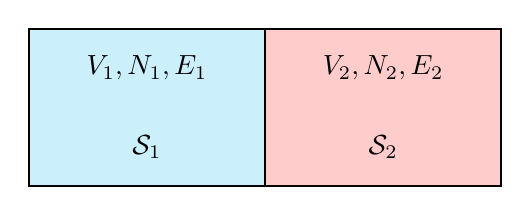
\begin{tikzpicture}

            \fill[cyan, fill opacity=0.2] (0,0) rectangle (3,2);
            \fill[red, fill opacity=0.2] (3,0) rectangle (6,2);

            \draw[thick] (0,0) rectangle (6,2);
            \draw[thick] (3,0) -- (3,2);

            \node at (1.5, 1.5) {$V_1, N_1, E_1$};
            \node at (4.5, 1.5) {$V_2, N_2, E_2$};
            \node at (1.5, 0.5) {$\mathcal{S}_1$};
            \node at (4.5, 0.5) {$\mathcal{S}_2$};

        \end{tikzpicture}
    \end{minipage}
    \hfill
    \begin{minipage}{0.45\textwidth}
        \[
            \begin{dcases}
                N = N_1 + N_2, \\
                V = V_1 + V_2, \\
                E = E_1 + E_2.
            \end{dcases}
        \]
    \end{minipage}
\end{figure}
Thermal contact means that the two systems can exchange energy, thus the total energy \(E\) is fixed, but the energy of each subsystem \(E_1\) and \(E_2\) can fluctuate. The total number of particles \(N\) and the total volume \(V\) are also fixed, since there is no exchange of matter or volume between the two systems.

The total energy can now be computed from the Hamiltonian of the system, sum of the subsystems' Hamiltonians plus an interaction term
\[
    H(\{q_j\},\,\{p_j\}) = H_1(\{q_{1j}\},\,\{p_{1j}\}) + H_2(\{q_{2j}\},\,\{p_{2j}\}) + \delta H_{12}(\{q_{1j}\},\,\{p_{1j}\},\,\{q_{2j}\},\,\{p_{2j}\}),
\]
where the last term accounts for the interaction between the two systems, which we will neglect in the following. The energy of the total system is fixed, but the energy of each subsystem can fluctuate. The probability of finding the system in a state with energy \(E_1\) is proportional to the number of states available to the second system with energy \(E_2 = E - E_1\). If we fix an energy shell of width \(\Delta\), we can write
\[
    E_k^{(1)} = k \Delta, \qquad E_k^{(2)} = E - E_k^{(1)} = E - k \Delta,
\]
and with this ``discretization'' we can count the number of states available to the total system at a fixed energy \(E\) as
\[
    \Gamma(E) = \sum_{k=0}^{E/\Delta} \Gamma_1(E_k^{(1)}) \Gamma_2(E-E_k^{(1)}),
\]
where \(\Gamma_k(E) = \int_{E < H_k < E + \Delta} \mathrm{d}\{q_{k}\} \mathrm{d}\{p_{k}\}\) is the number of states available to the \(k\)-th subsystem at energy \(E\).

Thus we are saying that \textit{in order to count the number of microstates at energy} \(E\) \textit{we have to multiply the number of microstates of the subsystem} \(S_1\) \textit{with energy} \(\epsilon_1\) \textit{to the number of microstates of} \(S_2\) \textit{at energy} \(\epsilon_2 = E - \epsilon_1\), \textit{then sum over all possible values of} \(\epsilon_1\).

The \textbf{most probable configuration} of the system is the one that maximizes the number of states available to the total system, which is equivalent to \textbf{maximizing the entropy} of the total system. Thus we can compute the entropy of the total system as
\[
    S(E) = k_B \log \left[ \sum_{k=0}^{E/\Delta} \Gamma_1(E_k^{(1)}) \Gamma_2(E-E_k^{(1)}) \right].
\]
Now, in order to maximize it, we can take the derivative of the entropy with respect to \(E_1\) and set it to zero: let us denote \(\bar{E}_1\) the energy of the subsystem \(S_1\) that maximizes the entropy, then \(\bar{E}_2 = E - \bar{E}_1\) is the energy of the subsystem \(S_2\) that maximizes the entropy. We have
\[
    \Gamma(\bar{E}^{(1)})\Gamma(\bar{E}^{(2)}) \leq \Gamma(E) \leq \frac{E}{\Delta} \Gamma(\bar{E}^{(1)})\Gamma(\bar{E}^{(2)}),
\]
where the first inequality comes from the fact that \(\Gamma(E)\) is a sum over all the values of \(E_1\), thus it is greater than or equal to the single term with \(E_1 = \bar{E}_1\), while the second inequality comes from the fact that there are at most \(E/\Delta\) terms in the sum, thus we can upper bound it by multiplying the maximum term by the number of terms. Taking the logarithm we arrive at
\[
    S(\bar{E}^{(1)}, V_1) + S(\bar{E}^{(2)}, V_2) \leq S(E, V) \leq S(\bar{E}^{(1)}, V_1) + S(\bar{E}^{(2)}, V_2) + k_B \log \left( \frac{E}{\Delta} \right),
\]
where both inequalities are saturated in the thermodynamic limit \(N \to \infty\): entropy and energy are extensive quantities, thus \(S(E, V) \sim N\) and \(E \sim N\), so the last term in the upper bound is negligible in the thermodynamic limit
\[
    k_B \log\left(\frac{E}{\Delta}\right) \sim k_B \log(N) \ll N \sim S(E, V).
\]
Thus we can write, in the thermodynamic limit, the entropy of the total system as the sum of the entropies of the subsystems, computed at the most probable values of the energy of the subsystems:
\[
    S(E,\,V) = S(\bar{E}^{(1)}, V_1) + S(\bar{E}^{(2)}, V_2).
\]

The first consequence of this result is that the \textbf{entropy is an extensive quantity}, since it scales with the number of particles \(N\) in the system. The second consequence is that the \textit{most probable configuration of the system is the one that maximizes the entropy}, which is equivalent to maximizing the number of states available to the total system. Thus we can write
\[
    \Gamma(E) = \Gamma_1(\bar{E}^{(1)}) \Gamma_2(\bar{E}^{(2)}).
\]
Therefore terms with different values of \(E_1\) are negligible compared to the term with \(E_1 = \bar{E}_1\), which is the one that maximizes the number of states available to the total system. This is a consequence of the fact that the number of states available to the total system grows exponentially with the number of particles \(N\), thus even a small difference in energy between different configurations can lead to a huge difference in the number of states available to the total system. \(\bar{E}^{(1)}\) and \(\bar{E}^{(2)}\) are the most probable values of the energy of the subsystems, which are the ones that maximize the entropy of the total system: the \textit{equilibrium energy values}. Mathematically, we can obtain \(\bar{E}^{(1)}\) from the saddle-point condition:
\[
    \frac{\partial}{\partial \epsilon} \left[ \Gamma_1(\epsilon) \Gamma_2(E - \epsilon) \right]_{\epsilon = \bar{E}^{(1)}} = 0,
\]
which, expanding the derivative, can be written as
\[
    \left[ \frac{\partial}{\partial \epsilon} \Gamma_1(\epsilon) \right]_{\epsilon = \bar{E}^{(1)}} \Gamma_2(E - \epsilon) + \Gamma_1(\epsilon) \left[ - \frac{\partial}{\partial \epsilon} \Gamma_2(\epsilon) \right]_{\epsilon = \bar{E}^{(2)}} = 0,
\]
which now, dividing by \(\Gamma_1(\bar{E}^{(1)}) \Gamma_2(\bar{E}^{(2)})\) (in order to build the logarithmic derivative), and using the definition of entropy we arrive at
\[
    \frac{\partial}{\partial \epsilon} S_1 (\epsilon) \bigg|_{\epsilon = \bar{E}^{(1)}} = \frac{\partial}{\partial \epsilon} S_2(\epsilon) \bigg|_{\epsilon = \bar{E}^{(2)}}.
\]
This is a fundamental result, which tells us that at equilibrium the derivative of the entropy with respect to the energy is the same for both subsystems. This allows us to define a thermodynamic quantity which is equal in systems in thermal equilibrium, called \textbf{temperature} \(T\) (recovering the first principle of thermodynamics). The temperature is defined as the inverse of the derivative of the entropy with respect to the energy, thus we can write
\begin{equation}
    \frac{1}{T} = \frac{\partial S}{\partial E}(E, V).
    \label{eq:temperature_definition}
\end{equation}

\subsection{Canonical Ensemble}

\begin{figure}[H]
    \begin{minipage}{0.5\textwidth}
        \centering
        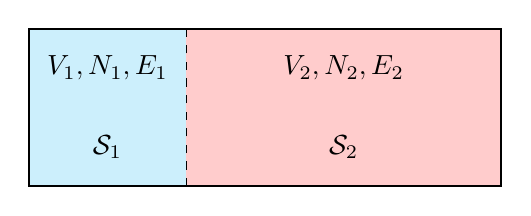
\begin{tikzpicture}

            \fill[cyan, fill opacity=0.2] (0,0) rectangle (2,2);
            \fill[red, fill opacity=0.2] (2,0) rectangle (6,2);

            \draw[thick] (0,0) rectangle (6,2);
            \draw[dashed] (2,0) -- (2,2);

            \node at (1, 1.5) {$V_1, N_1, E_1$};
            \node at (4, 1.5) {$V_2, N_2, E_2$};
            \node at (1, 0.5) {$\mathcal{S}_1$};
            \node at (4, 0.5) {$\mathcal{S}_2$};

        \end{tikzpicture}
    \end{minipage}
    \hfill
    \begin{minipage}{0.45\textwidth}
        \[
            \begin{dcases}
                N = N_1 + N_2, \\
                V = V_1 + V_2, \\
                E = E_1 + E_2,
            \end{dcases} \quad \text{and} \quad
            \begin{dcases}
                N_2 \gg N_1, \\
                V_2 \gg V_1, \\
                E_2 \gg E_1.
            \end{dcases}
        \]
    \end{minipage}
\end{figure}

The second system \(S_2\) is called the \textit{heat bath}, and it is so large that it can exchange energy with the first system \(S_1\) without changing its thermodynamic properties. The total system is isolated, thus we can apply the microcanonical ensemble to it. The probability of finding the system in a state with energy \(E_1\) is proportional to the number of states available to the second system with energy \(E_2 = E - E_1\), which is given by \(\Gamma_2(E - E_1)\).

Technically speaking, we want to find the probability distribution of the subsystem \(S_1\) when it is in contact with a heat bath \(S_2\), knowing the total probability distribution: the total system is isolated, thus we can apply the microcanonical ensemble to it, and we know that it will be evolving with a trajectory in the phase space that is uniformly distributed on the energy shell defined by the total energy \(E\). This means that if we analyze the evolution of the subsystem \(S_1\) in its phase space, we will find that it will not be limited to fixed energy states, but it will be able to explore all the energy states available to it, with a probability that is proportional to the number of states available to the heat bath \(S_2\) at the corresponding energy. We are interested in finding the \textbf{induced probability distribution} of the subsystem \(S_1\).

Let us visualize the phase space of the total system as a high-dimensional space, where each point represents a microstate of the total system. The energy shell defined by the total energy \(E\) is a hypersurface in this phase space, and the trajectory of the total system is uniformly distributed on this hypersurface. The subsystem \(S_1\) can be thought of as a projection of the total system onto a lower-dimensional subspace, where each point represents a microstate of the subsystem \(S_1\). The probability distribution of the subsystem \(S_1\) is then given by the projection of the uniform distribution on the energy shell onto this lower-dimensional subspace. Differents probabilities correspond to different energy states of the subsystem \(S_1\), and the probability of finding the subsystem \(S_1\) in a state with energy \(E_1\) is proportional to the number of states available to the heat bath \(S_2\) at energy \(E - E_1\).

The idea is to fix a point in the phase space of the subsystem \(S_1\) with energy \(E_1\), and then count the number of points in the phase space of the heat bath \(S_2\) that are compatible with this point, i.e. that have energy \(E - E_1\). This will give us the number of states available to the heat bath \(S_2\) at energy \(E - E_1\), which is proportional to the probability of finding the subsystem \(S_1\) in a state with energy \(E_1\).

So we fix an energy \(\epsilon\) for the subsystem \(S_1\), and we want to find the number of states available to the heat bath \(S_2\) at energy \(E - \epsilon\). \textit{The number of points in the phase space of} \(S\) \textit{that corresponds to} \(P\) \textit{is equal to the number of points in the phase space of} \(S_2\) \textit{that corresponds to} \(E - \epsilon\). Thus we can write
\[
    \rho(\{q_j\},\,\{p_j\}) \propto \frac{\Gamma_2(E - \epsilon)}{\Gamma(E)}.
\]
We know that the entropy of the heat bath \(S_2\) is related to the number of states available to it by the Boltzmann formula (we are using \(k_B=1\) for simplicity), such that
\[
    \Gamma_2(E - \epsilon) = e^{S_2(E - \epsilon)} \sim e^{S_2(E) - \frac{\partial S_2}{\partial E} \epsilon} = \Gamma_2(E)e^{-\frac{\partial S_2}{\partial E} \epsilon},
\]
where we have used the fact that the entropy is an extensive quantity, thus we can write it as a function of the energy per particle, and we have expanded it around the total energy \(E\) of the heat bath \(S_2\). We can now recall the temperature as a thermodynamic quantity defined as the inverse of the derivative of the entropy with respect to the energy, while reinserting the Boltzmann constant \(k_B\) for clarity, we have
\[
    \rho(\{q_j\},\,\{p_j\}) \propto e^{-\beta \epsilon} = e^{- \frac{\epsilon}{k_B T}},
\]
where \(\beta = \frac{1}{k_B T}\) is the inverse temperature. Thus we have derived the Boltzmann distribution for the subsystem \(S_1\) in contact with a heat bath \(S_2\). The probability of finding the subsystem \(S_1\) in a state with energy \(\epsilon\) is proportional to the exponential of the negative of the energy divided by the temperature of the heat bath \(S_2\). This is the canonical ensemble, where the subsystem \(S_1\) is in thermal equilibrium with a heat bath \(S_2\) at temperature \(T\).

We can now define the partition function \(\mathcal{Z}\) as the normalization constant for the probability distribution of the subsystem \(S_1\), such that
\begin{equation}
    \mathcal{Z} = \int \frac{\mathrm{d}^{3N}q \, \mathrm{d}^{3N}p}{h^{3N}N!} \, e^{-\beta H(\{q\},\,\{p\})},
    \label{eq:canonical_partition_function}
\end{equation}
which can be used as a generating function for the thermodynamic properties of the subsystem \(S_1\). For example, the free energy \(F\) can be computed from the partition function as
\begin{equation}
    F = -k_B T \log \mathcal{Z} = -\frac{1}{\beta} \log \mathcal{Z},
    \label{eq:canonical_free_energy}
\end{equation}
and the internal energy \(U\) can be computed as
\begin{equation}
    U = -\frac{\partial}{\partial \beta} \log \mathcal{Z},
\end{equation}
while the entropy \(S\) can be computed as
\begin{equation}
    S = -\frac{\partial F}{\partial T} = k_B \beta^2 \frac{\partial F}{\partial \beta}.
\end{equation}

\subsubsection{Discrete System}

A discrete system is a system that can only take a finite number of states, such as a spin system or a lattice gas. In this case, let us imagine a collection of \(N\) particles that can only occupy a finite number of states, let us imagine two values of spin, up and down, thus we have \(2^N\) possible configurations of the system. The phase space of the system is now a discrete set of points, configurations (a set of sets) \(\{c_j\}_{j=1}^N\), and the probability distribution of the system is defined on this discrete set of points.

Assuming that the phase space is explored uniformly at equilibrium, we can define the discretized version of the canonical and microcanonical ensembles, along with the corresponding observables, by replacing the integrals over the phase space with sums over the discrete set of points. The partition function can thus be written as a sum over all possible configurations of the system, such that
\begin{equation}
    \mathcal{Z} = \sum_{\{c_j\}} e^{-\beta H(\{c_j\})},
    \label{eq:discrete_partition_function}
\end{equation}
where the function \(H(\{c_j\})\) is the Hamiltonian of the system, which encodes the energy of each configuration of the system.

\section{Quantum Statistical Mechanics}

Let us complete the review of the theory background by recalling some basic concepts of quantum statistical mechanics, which is the extension of classical statistical mechanics to quantum systems.

Considering a general quantum mechanical system, we can study it with different tools, such as the hamiltonian operator, the density matrix, the partition function, etc. The Hamiltonian operator \(H\) is a self-adjoint operator that acts on the Hilbert space of the system, and it encodes the energy of the system. The density matrix \(\rho\) is a positive semi-definite operator that acts on the Hilbert space of the system, and it encodes the state of the system. The partition function \(\mathcal{Z}\) is a scalar quantity that encodes the thermodynamic properties of the system.

\subsection{Hilbert Space and Dynamics}

In a quantum system, the state of the system is described by a vector \(\ket{\psi}\) in the \textbf{Hilbert space} \(\mathcal{H}\), and the observables of the system are described by self-adjoint operators that act on the Hilbert space. The dynamics of the system is governed by the \textit{Schrödinger equation}, which describes how the state of the system evolves in time under the action of the \textbf{Hamiltonian operator}, which is a self-adjoint operator that encodes the energy of the system. Since the Hamiltonian operator is self-adjoint, it has a complete set of eigenstates \(\{\ket{E_n}\}_{n=1}^D\) with corresponding eigenvalues \(\{E_n\}_{n=1}^D\) (\(D\) is the dimension of the Hilbert space), which represent the energy levels of the system:
\[
    \hat{H} \ket{E_n} = E_n \ket{E_n}.
\]
Given a state \(\ket{\psi}\) of the system and a complete set of eigenstates of the Hamiltonian, we can express the state \(\ket{\psi}\) as a linear combination of the eigenstates of the Hamiltonian as
\[
    \{\ket{E_n}\}_{n=1}^D \implies \ket{\psi} = \sum_{n=1}^D c_n \ket{E_n},
\]
where \(c_n = \bra{E_n} \ket{\psi} \in \mathbb{C}\) are the coefficients of the linear combination, which can be interpreted as the probability amplitudes of the state \(\ket{\psi}\) in the energy eigenbasis. Indeed they respect the normalization condition \(\sum_{n=1}^D |c_n|^2 = 1\), which ensures that the total probability of finding the system in any of the energy eigenstates is equal to one.

We have to note that dealing with quantum statistical mechanics is more complicated than dealing with classical statistical mechanics, since we have to deal with operators instead of functions, and we have to deal with the non-commutativity of operators. However, the general principles of statistical mechanics still apply, and we can still define ensembles, partition functions, and thermodynamic quantities in the quantum case. The main difference is that we have to use the language of operators and Hilbert spaces instead of the language of functions and phase space.

\subsubsection{Observables and Expectation Values}

Recalling finally that the observables are associated to hermitian operators, the \textbf{expectation value} of an observable \(\hat{A}\) in the state \(\ket{\psi}\) can be computed as
\[
    \bra{\psi} \hat{A} \ket{\psi} = \sum_{n,m} c_n^* c_m \bra{E_n} \hat{A} \ket{E_m}.
\]
If we were to consider the time evolution of the state \(\ket{\psi}\) under the action of the Hamiltonian, we can write it as
\[
    \ket{\psi(t)} = \sum_{n} c_n(t) \ket{E_n}, \quad c_n(t) = c_n e^{-i \frac{E_n}{\hbar} t},
\]
and thus the expectation value of an observable \(\hat{A}\) at time \(t\) can be computed as
\[
    \bra{\psi(t)} \hat{A} \ket{\psi(t)} = \sum_{n,m} c_n^*(t) c_m(t) \bra{E_n} \hat{A} \ket{E_m} = \sum_{n,m} c_n^* c_m e^{i \frac{E_n - E_m}{\hbar} t} \bra{E_n} \hat{A} \ket{E_m},
\]
which is a complicated time dependent sum over the energy eigenstates of the system, but quantum statistical mechanics allows us to simplify it under some assumptions which we will see in the following.

However, we can alreadty use the fact that the theory applies at equilibrium, where \uline{observables are time independent up to small fluctuations}; in order to avoid such complications, we can consider the \textbf{time average} of the expectation value of an observable \(\hat{A}\) over a \textit{long time interval} \(T\).\footnote{With long time interval here we refer to larger time scales than the microscopic ones, but still much smaller than the macroscopic time scale.} We denote the time average of an observable \(\hat{A}\) as \(\overline{\bra{\psi(t)} \hat{A} \ket{\psi(t)}}\), and we can compute it as
\[
    \bra{\psi(t)} \hat{A} \ket{\psi(t)} \mapsto \overline{\bra{\psi(t)} \hat{A} \ket{\psi(t)}}.
\]

\subsection{Postulates of Quantum Statistical Mechanics}

We can now introduce the postulates of quantum statistical mechanics, which are the fundamental principles that govern the behavior of quantum systems at thermal equilibrium. These postulates are based on the idea that at thermal equilibrium, the system is in a state that maximizes the entropy of the system, subject to the constraints imposed by the energy and other conserved quantities of the system. For a macroscopic quantum system with energy \(E\) at thermal equilibrium, the following holds:
\begin{itemize}
    \item \textbf{Postulate of equal a priori probabilities}: in an isolated system, all microstates are equally probable, thus the probability distribution of the system is uniform over the energy shell defined by the energy \(E\) and a small energy interval \(\Delta\), such that we can write
          \[
              \overline{\vert c_n \vert}^2 = \begin{dcases}
                  \frac{1}{D}, & \text{if } E_n \in [E, E + \Delta], \\
                  0,           & \text{otherwise},
              \end{dcases}
          \]
          where \(D\) is the number of energy eigenstates in the energy shell defined by \(E\) and \(\Delta\) (the dimension of the Hilbert space in which the system is described).

    \item \textbf{Postulate of random phases}: the phases of the coefficients \(c_n\) are random variables uniformly distributed in the interval \([0, 2\pi]\), thus
          \[
              \overline{c_n(t) c_m^*(t)} = \frac{1}{T} \int_0^T \mathrm{d}t \, c_n^*(t) c_m(t) = \frac{1}{T}  \int_0^T \mathrm{d}t \, c_n^* c_m \, e^{i \frac{E_n - E_m}{\hbar} t} = \begin{dcases}
                  \vert c_n \vert^2, & \text{if } n = m, \\
                  0,                 & \text{otherwise},
              \end{dcases}
          \]
          which in the end explains our previous assumption on expectation values of observables at equilibrium.
\end{itemize}

It is still an open question to justify these postulates from first principles, but they are very useful for computing the thermodynamic properties of quantum systems at thermal equilibrium, and they are widely used in the literature of quantum statistical mechanics.

Using these postulates, we can compute the time average of an observable \(\hat{A}\) using the expression for the expectation value of an observable at time \(t\) that we have derived before, thus we can write
\[
    \begin{aligned}
        \overline{\bra{\psi(t)} \hat{A} \ket{\psi(t)}} = \frac{1}{T} \int_0^T \mathrm{d}t \, \bra{\psi(t)} \hat{A} \ket{\psi(t)} = \sum_{n} |c_n|^2 \bra{E_n} \hat{A} \ket{E_n},
    \end{aligned}
\]
where in the end we have used the postulate of random phases to eliminate the off-diagonal terms in the sum, thus we are left with a sum over the diagonal terms only, which is a much simpler expression to compute. This is a fundamental result, which tells us that at thermal equilibrium, the expectation value of an observable \(\hat{A}\) can be computed as a sum over the energy eigenstates of the system, weighted by the probability of finding the system in each energy eigenstate:
\[
    \overline{\bra{\psi(t)} \hat{A} \ket{\psi(t)}} = \sum_{n \in I(E)} \vert c_n \vert^2 A_{nn}, \quad I(E) = \{n : E \leq E_n \leq E + \Delta\}.
\]

\subsection{Density Matrix and Statistical Ensembles}

After these considerations, we are directly led to the definition of a statistical ensemble for a quantum system at thermal equilibrium, which is a probability distribution over the energy eigenstates of the system, such that the probability of finding the system in an energy eigenstate \(\ket{E_n}\) is given by \(\vert c_n \vert^2\). Since we have derived a sort of microcanonical ensemble for the quantum system from the postulates of quantum statistical mechanics, we have to define a sort of uniform distribution over the energy eigenstates in the energy shell defined by \(E\) and \(\Delta\). We can accomplish this by defining \textbf{density matrix}, which is a positive semi-definite operator that encodes the state of the system, and it can be used to compute the expectation values of observables and the thermodynamic properties of the system.

We can define the density matrix \(\hat{\rho}\) for the quantum microcanonical ensemble as
\[
    \hat{\rho} = \frac{1}{Z} \sum_{E \leq E_n \leq E+\Delta} \ket{E_n} \bra{E_n},
\]
where \(Z\) is just a normalization constant. The expectation value of an observable \(\hat{A}\), with this definition of the density matrix, can be then computed as
\[
    \langle \hat{A} \rangle \sim \overline{\bra{\psi(t)} \hat{A} \ket{\psi(t)}} = \mathrm{Tr}[\hat{\rho} \hat{A}].
\]

\begin{remark}
    An useful property of the density matrix, coming from the fact that the coefficients \(c_n\) are random variables respecting the normalization condition \(\sum_n \vert c_n \vert^2 = 1\), is that its trace is equal to one:
    \[
        \Tr \hat{\rho} = \sum_n \bra{E_n} \hat{\rho} \ket{E_n} = \sum_n \vert c_n \vert^2 = 1,
    \]
    which ensures that the total probability of finding the system in any of the energy eigenstates is equal to one.
\end{remark}

Defining an ensemble in quantum statistical mechanics automatically defines a density matrix, which encodes the state of the system, and from which we can compute the expectation values of observables and the thermodynamic properties of the system. We are governing our set of eigenstates with a probability distribution, which is encoded in the density matrix, and we can compute the expectation values of observables and the thermodynamic properties of the system from this density matrix.

Indeed, we can also define the canonical ensemble for a quantum system at thermal equilibrium, by defining the density matrix for the canonical ensemble as
\[
    \hat{\rho} = \frac{1}{\mathcal{Z}} e^{-\beta \hat{H}} = \frac{1}{\mathcal{Z}} \sum_{n} e^{-\beta E_n} \ket{E_n} \bra{E_n},
\]
where now \(\mathcal{Z}\) is still a normalization constant, but it has a non trivial expression which recovers its definition as the partition function of the system, which can be computed recalling \(\Tr \hat{\rho} = 1\) as
\[
    \mathcal{Z} = \Tr e^{-\beta \hat{H}} = \sum_n e^{-\beta E_n},
\]
and it is known as the \textbf{thermal partition function}.

\subsubsection{Free Energy and Thermodynamic Observables}

Finally, we can state one last postulate of quantum statistical mechanics, which is the identification of the thermodynamic free energy \(F\) with the partition function \(\mathcal{Z}\):
\[
    F = -k_B T \log \mathcal{Z} = -\frac{1}{\beta} \log \mathcal{Z},
\]
which is the same relation that we have in classical statistical mechanics. These postulates are like operational tools: justify them as they are can be rally difficult and it is an actual field of research with a lot of literature, but they are very useful for computing the thermodynamic properties of quantum systems at thermal equilibrium. For us, justifying why a precise postulate work in the actual setting will be enough.

As usual, from the free energy we can compute all the thermodynamic observables of the system, such as the internal energy \(U\) and the entropy \(S\), with the standard relations that we have in classical statistical mechanics. This is the power of such postulates: they allow us to compute the thermodynamic properties of quantum systems at thermal equilibrium, and they are widely used in the literature of quantum statistical mechanics.